\documentclass{report}
% Packages
\usepackage{import}
\usepackage{xcolor}
\usepackage{cancel}
\usepackage{mathtools}
\usepackage{hyperref}
\usepackage{setspace}
\usepackage{float}
\usepackage{parskip}
\setlength{\parindent}{0pt}
\usepackage{scalerel}

\renewcommand{\vec}{\mathbf}
\DeclareMathOperator{\vectorprojection}{proj}
\NewDocumentCommand{\proj}{s e{_} m}{%
    \IfBooleanTF{#1}{#3_{\stretchrel*{\parallel}{\perp}#2}}{\vectorprojection_{#2}#3}
}
\renewcommand{\Re}{\operatorname{Re}}
\renewcommand{\Im}{\operatorname{Im}}
\renewcommand{\Arg}{\operatorname{Arg}}
\newcommand{\Span}{\operatorname{span}}
\newcommand{\Dim}{\operatorname{dim}}
\newcommand{\Ker}{\operatorname{ker}}
\newcommand{\Image}{\operatorname{im}}
\newcommand{\Nullity}{\operatorname{nullity}}
\newcommand{\Rank}{\operatorname{rank}}
\newcommand{\Det}{\operatorname{det}}
\newcommand{\Var}{\operatorname{Var}}
\newcommand{\Exp}{\operatorname{Exp}}

% augmented matrix
\newenvironment{amatrix}[1]{%
  \left(\begin{array}{@{}*{#1}{c}|c@{}}
}{%
  \end{array}\right)
}

% Custom perms and combs commands
\newcommand\Myperm[2][^n]{\prescript{#1\mkern-2.5mu}{}P_{#2}}
\newcommand\Mycomb[2]{\prescript{#1\mkern-0.5mu}{}C_{#2}}
% Custom column vector command
\newcommand{\cvec}[1]{ \begin{pmatrix} #1 \end{pmatrix} }
% Custom determinant command
\newcommand{\det}[1]{ \begin{vmatrix} #1 \end{vmatrix} }

% Colors
\definecolor{yorhabg}{HTML}{131314}
\definecolor{yorhafg}{HTML}{C9C7CD}
\definecolor{yorhagrid}{HTML}{B5AF9C}
\definecolor{mred}{HTML}{D67069}
\definecolor{mblue}{HTML}{6887A1}

\usepackage[dvipsnames]{xcolor}
\definecolor{pastel_red}{RGB}{255, 173, 173}
\definecolor{pastel_orange}{RGB}{255, 214, 165}
\definecolor{pastel_yellow}{RGB}{253, 255, 182}
\definecolor{pastel_green}{RGB}{176, 217, 176}
\definecolor{pastel_blue}{RGB}{167, 199, 231}
\definecolor{pastel_purple}{RGB}{222, 218, 244}

\pagecolor{yorhabg}		% Set background color
\color{yorhafg}

\import{preamble.sty}

\usepackage[T1]{fontenc}			% Font package

\usepackage{fouriernc}

\usepackage{sectsty}
\usepackage{graphicx}
\usepackage{amsmath}
\usepackage{amsfonts}
\usepackage{amssymb}
\usepackage[skins, most]{tcolorbox}

\DeclareMathOperator{\sgn}{sgn}

\usepackage{tikz}
\usepackage{eso-pic}
\usetikzlibrary{calc, shadows.blur}
\usetikzlibrary{angles, quotes}
\usetikzlibrary{3d}

% Margins
\topmargin=0in
\evensidemargin=0in
\oddsidemargin=0in
\textwidth=6.5in
\textheight=9.0in
\headsep=0.25in

\AtBeginEnvironment{tcolorbox}{\small}

\newtcolorbox{imp}{enhanced,arc=0mm,colback=yorhabg,colframe=mred,leftrule=10mm,coltext=yorhafg,%
overlay={\node[anchor=west,outer sep=2pt] at (frame.west) {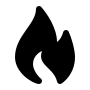
\includegraphics[width=6mm]{images/imageb.png}}; }}

\newtcolorbox{shortcut}{enhanced,arc=0mm,colback=yorhabg,colframe=mred,leftrule=10mm,coltext=yorhafg, coltitle=yorhabg, title=\texttt{Shortcut.}, 
overlay={\node[anchor=west,outer sep=2pt] at (frame.west) {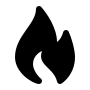
\includegraphics[width=6mm]{images/imageb.png}}; }}

\newtcolorbox{question}[1]{
    enhanced, 
    colback=yorhabg,
    colframe=mblue,
    coltext=yorhafg,
    coltitle=yorhabg,
    attach boxed title to top left={yshift*=-\tcboxedtitleheight}, 
    title=\texttt{#1},
    boxed title size=title,
    boxed title style={%
        rounded corners=northeast, 
        rounded corners=northwest, 
        colback=tcbcolframe, 
        boxrule=0pt,
    },
    underlay boxed title={%
        \path[fill=tcbcolframe] (title.south west)--(title.south east) 
            to[out=0, in=180] ([xshift=5mm]title.east)--
            (title.center-|frame.east)
            [rounded corners=5pt] |- 
            (frame.north) -| cycle; 
    },
}

\newcommand\bb[1]{\textcolor{yorhafg}{\textbf{#1}}}

% Spacing
\setlength{\jot}{1.5em}
\setlength{\thickmuskip}{10}
\setlength{\medmuskip}{7}
\setlength{\thinmuskip}{5}
\setstretch{1.25}

\makeatletter
\renewcommand*\env@matrix[1][*\c@MaxMatrixCols c]{%
  \hskip -\arraycolsep
  \let\@ifnextchar\new@ifnextchar
  \array{#1}}
\makeatother

\title{\textbf{MATH1141: Higher Mathematics 1B - Algebra}}
\author{L. Cheung}
\date{\today}

\begin{document}

\maketitle
\tableofcontents
\newpage

\chapter{Vector Spaces}

	A field in a non-empty set $\mathbb{F}$ which has two binary operations $+$, $\cdot$, and satisfies all 12 number laws.

	\section{Examples of fields}

		\begin{itemize}
			\item $\mathbb{Q}, \mathbb{R}, \mathbb{C}$
			\item $\mathbb{Q}(\sqrt{3}) \coloneq \left\{ a + b\sqrt{3} \;|\; a,b \in \mathbb{Q}\right\}$
			\item $\mathbb{Q}(i) \coloneq \left\{a + bi \;|\; a,b \in \mathbb{Q}\right\}$, where $i = \sqrt{-1}$
			\item Every prime number $p$ defines a field
				\begin{align*}
					\mathbb{F}_p = GF(p) \coloneq {0,1,2,...,p-1}
				\end{align*}
		\end{itemize}

	\section{Definition of Vector Space}

		A vector space over a field $F$ (the set of scalars) is a non-empty set $V$ of elements, vectors, for which addition and scalar multiplication are defined and which obey the following 10 axioms.
		
		\begin{enumerate}
			\item \textbf{Closure under addition}: adding two vectors yields a vector.
			\item \textbf{Associative law of addition}: $(\vec{u} + \vec{b}) + \vec{w} = \vec{u} + (\vec{b} + \vec{w})$.
			\item \textbf{Commutative law of addition}: $\vec{u} + \vec{v} = \vec{v} + \vec{u}$.
			\item \textbf{Existence of zero}: there is an element $\vec{0}$ in $V$ called the zero vector that satisfies the property $\vec{v} + \vec{0} = \vec{v},\; \forall \vec{v} \in V$.
			\item \textbf{Existence of negative}: for each $\vec{v} \in V$ there exists an element $\vec{w} \in V$ such that $\vec{v} + \vec{w} = \vec{0}$.
			\item \textbf{Closure under scalar multiplication}: for all $\vec{v} \in V$ and $\lambda \in \mathbb{F}$, $\lambda \vec{v} \in V$.
			\item \textbf{Associative law of scalar multiplication}: for all $\lambda, \mu \in \mathbb{F}$ and $\vec{v} \in V$,
				\begin{align*}
					\lambda ( \mu \vec{v} ) = ( \lambda \mu ) \vec{v}.
				\end{align*}
			\item For all $\vec{v} \in  V$, $1 \vec{v} = \vec{v}$.
			\item \textbf{Scalar distributive law}: for all $\lambda, \mu \in \mathbb{F}$ and $\vec{v} \in V$,
				\begin{align*}
					( \lambda + \mu ) \vec{v} = \lambda \vec{v} + \mu \vec{v}.
				\end{align*}
			\item \textbf{Vector distributive law} for all $\lambda \in \mathbb{F}$ and $\vec{u}, \vec{v} \in V$,
				\begin{align*}
					\lambda (\vec{u} + \vec{v}) = \lambda \vec{u} + \lambda \vec{v}.
				\end{align*}
		\end{enumerate}

		\textcolor{pastel_yellow}{Note}: addition in the field and addition in the vector space is different, however this is not distinguished in notation.
		\begin{itemize}
			\item Axioms 1-5 say that $(V, +)$ is an abelian group
			\item Axioms 6-8 describe how $\mathbb{F}$ acts on $V$
			\item Axioms 9 and 10 describe that addition and scalar multiplication are compatible.
		\end{itemize}
		\textcolor{pastel_yellow}{Note}: each axiom (except for 4) are "for all" statements, and apply to all

	\section{Basic Properties}

		In any vector space $V$, the following properties hold

		\begin{enumerate}
			\item \textbf{Uniqueness of Zero}: There is one and only one zero vector

				\textcolor{pastel_blue}{Proof}: If $\vec{0}' \in V$ satisfies $\vec{v} + \vec{0}' = \vec{v}$ for all $\vec{v} \in V$, then
					\begin{align*}
						\vec{0}' = \vec{0}' + \vec{0} = \vec{0} + \vec{0}' = \vec{0}.
					\end{align*}

			\item \textbf{Cancellation Property}: If $\vec{u},\vec{v},\vec{w} \in V$ satisfy
				\begin{align*}
					\vec{u} + \vec{v} = \vec{u} + \vec{w}, \text{ then } \vec{v} = \vec{w}.
				\end{align*}

			\item \textbf{Uniqueness of Negatives}
		\end{enumrate}

		\subsection{Additional basic properties}

			Suppose that $\vec{v}$ is a vector in a vector space $V$; $\lambda$ is a scalar; $0$ is the zero scalar; $\vec{0}$ is the zero vector in $V$. Then the following properties hold.

			\begin{itemize}
				\item $\lambda \vec{0} = \vec{0},$
				\item $0 \vec{v} = 0$.
				\item $(-1) \vec{v} = -\vec{v}$. (Here, $-1$ is a scalar and $-\vec{v}$ is the additive inverse of $\vec{v}$).
				\item If $\lambda \vec{v} = \vec{0}$, then either $\lambda = 0$ or $\vec{v} = \vec{0}$.
				\item If $\lambda \vec{v} = \mu \vec{v}$, and $\vec{v} \neq \vec{0}$, then $\lambda = \mu$.
			\end{itemize}

	\section{Standard Examples}

		\textbf{Example 1}

		The set $\mathbb{F}^n = \left\{\cvec{a_1\\a_2\\\vdots\\a_n}: a_i \in \mathbb{F} \forall i \right\}$ is a vector space over $\mathbb{F}$ under the usual (component-wise) addition and multiplication by a scalar.

		\textbf{Example 2}

		The set $M_{m,n}(\mathbb{F})$ of all $m \times n$ matrices with entries in $\mathbb{F}$ is a vector space over $\mathbb{F}$.
		
		\textbf{Example 3}

		Let $X$ by any non-empty set. The set  $\mathcal{F}[X] = {f: X \rightarrow \mathbb{F}}$ of all $\mathbb{F}$-valued functions with domain $X$ is a vector space over $\mathbb{F}$ with point-wise addition and scalar multiplication.

		To prove that a system $V$ is a vector space, every axiom must be verified. To prove that $V$ is not a vector space, only one axiom needs to be disproven.
		
\chapter{Standard Examples and Subspaces}	

	There are subsets of $\mathcal{R}[\mathbb{R}]$ that are also vector spaces.

	The substructures of a field are called subfields. More precisely:

	\begin{question}{Definition}
		If $\mathbb{K}$ is a field, then a subset $\mathbb{F} \subseteq \mathbb{K}$ is called a subfield of $\mathbb{K}$, denoted by $\mathbb{F} \leq \mathbb{K}$, if $\mathbb{F}$ is also a field with the same $+$ and $\cdot$ as in $\mathbb{K}$.
	\end{question}
	\begin{question}{Definition}
		Let $V$ be a vector space over a field $\mathbb{F}$. A subset $S \subseteq V$ is called a subspace of $V$ if $S$ is itself a vector space over $\mathbb{F}$ with the same operations for addition and scalar multiplication.

		If $S$ is a subspace of $V$, then $S$ contains the zero vector $\vec{0}_V$ of $V$. Hence, if $\vec{0}_V \notin S$, then $S$ is not a subspace. Ie. a subspace must have the unique zero vector of its larger space.
	\end{question}

	\textbf{Example}
		
		Consider $\mathbb{R}^3$ as a vector space over $\mathbb{R}$.

		\begin{enumerate}
			\item ${\vec{0}}$ is a subspace. $\mathbb{R}^3$ itself is a subspace.
			\item Any line through the origin $\vec{0}$ is a subspace.
			\item Any plane through the origin is a subspace.
		\end{enumerate}

		These are the only subspaces in $\mathbb{R}^3$
		

	\section{The Subspace Theorem}
	\begin{question}{Theorem}
		A subset $S$ of a vector space $V$ over $\mathbb{F}$ is a subspace if and only if

		\begin{itemize}
			\item $\vec{0} \in S$,
			\item $\vec{u} + \vec{v} \in S$ for all $\vec{u}, \vec{v}, \in S$, and
			\item $\lambda \vec{v} \in S$ for all $\vec{v} \in S$, scalars \lambda \in \mathbb{F}.
		\end{itemize}

		Alternatively,

		\begin{itemize}
			\item $\vec{0}_V \in S$, and
			\item $\lambda \vec{u} + \vec{v} \in S$, and scalars $\lambda \in \mathbb{F}$.
		\end{itemize}
	\end{question}

	Note: the only subspaces of $\mathbb{R}^2$ are lines that pass through the origin, ie. contain the zero vector.

	\begin{question}{Example}
		For which values $a \in \mathbb{R}$ is the set $S_a = \left\{y \in \mathcal{R}[\mathbb{R}] : \frac{d^2y}{dx^2} + 3 \frac{dy}{dx} + 4y = a\right\}$ a subspace of $\mathcal{R}[\mathbb{R}] $?
		\\ \\
		Since the zero vector is not defined for values of $a$ other than 0, the only solution is $a = 0$.
	\end{question}

	\textbf{Finding all subspaces of $\mathbb{F}^n$}

		Suppose $W \leq \mathbb{F}^n$. Then $\vec{0} \in W$. So
		\begin{itemize}
			\item either $W = {\vec{0}}$ or $\exists \vec{u} \in W,\; \vec{u} \neq 0$. Then all scalar multiples of $\vec{u}$ are in $W$. Thus, $\left{\lambda \vec{u} \;|\; \lambda \in \mathbb{F}}$
			\item Thus, either $W = \left\{ \lambda \vec{u} \;|\; \lambda \in \mathbb{F} \right\}$ or $\exists \vec{v} \in W$ with $\vec{v} \neq \lambda \vec{u}$ for all $\lambda \in \mathbb{F}$. So \left\{ \lambda \vec{u} + \mu \vec{v} \;|\; \lambda, \mu \in \mathbb{F} \right\} \leq W. Hence,
			\item either $W = \left\{ \lambda \vec{u} + \mu \vec{v} \;|\; \lambda, \mu \right\}$ or $\exists \vec{w} \in W$ with $\vec{w} \neq \lambda \vec{u} + \mu \vec{v}$ for all $\lambda, \mu$. Thus, $\left\{ \lambda \vec{u} + \mu \vec{v} + \nu \vec{w} \;|\; \lambda, \mu, \nu \in \mathbb{F} \right\} \leq W$
			\item If $n = 3$, then $W = \left\{ \lambda\vec{u} + \mu\vec{v} + \nu\vec{w} \;|\; \lambda, \mu, \nu \in \mathbb{F} \right\}$. If $n > 3$, we may continue this construction.
		\end{itemize}

\chapter{Lin. Combination and Lin. Span}

	\section{Linear Combination}

		Let $V$ be a vector space. We can form a vector in $V$ by adding up scalar multiples of finitely many vectors $\vec{v_1},\dots\vec{v_n}$ in $V$. Such a vector is called a linear combination of $\vec{v_1}, \dots \vec{v_n}$
		\begin{question}{Definition}
			A linear combination of finitely many vectors $\vec{v_1}, \dots \vec{v_n}$ in a vector space $V$ over $\mathbb{F}$ is a sum of scalar multiples of the form.
			\begin{align*}
				\lambda_1 \vec{v_1} + \dots + \lambda_n \vec{v_n} \text{ with } \lambda_1, \dots, \lambda_n \in \mathbb{F}.
			\end{align*}
		\end{question}

		\begin{question}{Example}
			Consider the subspace
			\begin{align*}
				S = \left\{p \in \mathbb{P}_2(\mathbb{R}) \;|\; xp'(x) = 2p(x) \forall x \in \mathbb{R}\right\} \leq \mathbb{P}_2(\mathbb{R})
			\end{align*}
		\end{question}
	
	\section{Linear Span and Spanning Set}

		\begin{question}{Definition}
			Let $S$ be a subset of a vector space $V$. Then the span of $S$ is the set $\Span(S)$ of all linear combinations of vectors in $S$:
			\begin{align*}
				\Span(S) = \left\{ \lambda_1\vec{v_1} + \cdots + \lambda_n\vec{v_n} \;\middle| \begin{array}{l}\vec{v_1},\dots,\vec{v_n} \in S \\ \lambda_1,\dots,\lambda_n \in \mathbb{F} \end{array}, \; \forall n \in \mathbb{N}\right\}
			\end{align*}

			If $S = \left\{\vec{v_1},\dots,\vec{v_n}\right\}$, then we write $\text{span}(S) = \text{span}\left\{\vec{v_1},\dots\vec{v_n}\right\}$. If $\text{span}(S) = V$, $S$ is called a spanning set of $V$.
		\end{question}

		\begin{question}{Example}
			Let $S$ be a nonempty subset of a vector space $V$. Then $\Span(S)$ is a subspace of $V$, and it is the smallest subspace containing $S$.
			\\ \\
			First, for any $\mathbb{v} \in S,\; \vec{0} = 0\vec{v} \in \Span(S)$.
			If $\vec{v},\vec{u} \in \Span(S)$, then $\vec{v} = \lambda_1 \vec{v_1} + \dots + \lambda_n \vec{v_n}$ and $\vec{u} = \mu_1 \vec{u_1} + \dots + \mu_m \vec{u_m}$ for some $\vec{v_i}, \vec{u_i} \in S$ and $\lambda_i, \mu_i \in \mathbb{F}$. Thus, if $\lambda \in \mathbb{F}$, then
			\begin{align*}
				\lambda\vec{v} + \vec{u} &= \lambda(\lambda_1\vec{v_1} + \dots + \lambda_n\vec{v_n}) + \mu_1\vec{u_1} \dots + \mu_m\vec{u_m}	\\
										 &= (\lambda \lambda_1) \vec{v_1} \dots + (\lambda \lambda_n) \vec{v_n} + \mu_1\vec{u_1} \dots + \mu_m\vec{u_m}
			\end{align*}
			is a linear combination of vectors in $S$. Hence, $\lambda\vec{v} + \vec{u} \in \Span(S)$, proving $\Span(S) \leq V$ by the alternative subspace test.
		\end{question}.

		\begin{question}{Example}
			What is the geometric interpretation of $\Span \left\{\cvec{1\\2\\-1},\cvec{1\\1\\-1}\right\}$ in $\mathbb{R}^3$?

			It is a plane through the origin with parametric vector form
			\begin{align*}
				\vec{x} = \lambda \cvec{1\\2\\-1} + \mu \cvec{1\\1\\-1}
			\end{align*}
		\end{question}

		\begin{question}{Example}
			Let $\vec{u} = \cvec{0\\1\\0}, \vec{v} = \cvec{1\\4\\1} \in \mathbb{R}^3$, and the set $S = \left\{\cvec{1\\3\\4},\cvec{1\\2\\3}\right\}$. Is $\vec{u} \in \Span(S)$
			\\ \\
			Check there exists scalars $\lambda, \mu \in \mathbb{R}$ such that
			\begin{align*}
				\lambda \cvec{1\\3\\4} + \mu \cvec{1\\2\\3} = \cvec{0\\1\\0} \quad \text{ or } \quad \cvec{1&1\\3&2\\4&3} \cvec{\lambda\\\mu} = \cvec{0\\1\\0}
			\end{align*}
			Thus, we need to test the solvability of a linear system $A\vec{x} = \vec{b}$ with augmented matrix $\begin{amatrix}{2}
				1 & 1 & 1 \\
				3 & 2 & 0 \\
				4 & 3 & 1
			\end{amatrix}$.
			The matrix can be reduced into row echelon form
			\begin{align*}
				\begin{amatrix}{2}
					1 & 1 & 1	\\
					0 & -1 & 3	\\
					0 & 0 & 0	
				\end{amatrix}.
			\end{align*}
			A solution to the system exists, meaning that $\vec{u} \in \Span(S)$. We substitute back to find $\lambda$ and $\mu$, providing $\mu = 3$ and $\lambda = 1 - \mu = -2$.

		\end{question}

		It can also be applied to find an arbitrary vectors. By solving the linear combination of the vectors in the span for $\vec{b}$, a generalised solution for the span can be found.

		Suppose $S = \left\{\vec{v_1},\dots,\vec{v_n}$ and a vector $\vec{b}$ are all in $\mathbb{F}^m$. Then $\vec{b} \in \Span(S)$ if and only if there are scalars $\vec{x_1,\dots,x_n}$ such that
			\begin{align*}
				x_1\vec{v_1} + \dots + x_n\vec{v_n} = \vec{b}.
			\end{align*}

\chapter{Linear Dependence/Independence}

	\begin{question}{Example}
		Does $\sin^2x$ lie in the span of $\{1, \cos^2x\}$ inside $C(\mathbb{R})$?
		\\ \\
		Yes, $\sin^2x = 1 - \cos^2x$
	\end{question}

	\begin{question}{Example}
		Does $e^x$ lie in the span of $\{1,x,x^2,\dots\}$ inside $C(\mathbb{R})$?
		\\ \\
		No, exponential functions grow faster than any polynomial.
	\end{question}

	\begin{question}{Definition}
				The subspace of $\mathbb{F}^m$ spanned by the columns of an $m \times n$ matrix $A$ is called the column space of $A$ and is denoted by $\mathcal{C}(A)$. The subspace $\mathcal{N}(A)$ of the solutions of $A\vec{x} = \vec{0}$ is called the null space of $A$.
				\\
				If a vector can be written as a scalar multiple of any of the columns in the matrix, it is in the column space.
	\end{question}


	Suppose $S \subset V$. If we can remove a vector from the set $S$ without changing the span, then the set $S$ is said to be linearly dependent. Otherwise the set is linearly independent.

	If $\vec{0} \in S$, then $S$ is linearly dependent.

	If $S$ is a spanning set of $V$ and $\vec{v} \in V - S$, then $S \cup \{\vec{v}\}$...

	\subsubsection{Testing Linear Dependence/Independence}
		
		\begin{question}{Example}
			\begin{align*}
				S_1 = \left\{ \cvec{2\\-2},\cvec{-1\\1} \right\}, \quad S_2 = \left\{ \cvec{2\\-2\\-1}, \cvec{-1\\1\\3} \right\}, \quad S_3 = S_u \cup \left\{\cvec{1\\-1\\7}\right\}
			\end{align*}
			\begin{itemize}
				\item $S_1$ is linearly dependent
				\item $S_2$ is linearly independent
				\item $S_3$ no vector is a scalar multiple of the other, but the sum of two make the third, therefore it is linearly dependent
			\end{itemize}
		\end{question}

		\begin{question}{Definition}
			Let $S$ be a subset of a vector space.

			\begin{enumerate}
				\item If there exist distinct vectors $\vec{v_1}, \dots, \vec{v_n} \in S$ and scalars $\lambda_1, \dots, \lambda_n$, not all zero, such that 
					\begin{align*}
						\lambda_1\vec{v_1} + \dots + \lambda_n\vec{v_n} = \vec{0},
					\end{align*}
					then we say that $S$ is linearly dependent.
				\item If the opposite case is true, that is that the only solution for the linear combination of vectors in $S = \vec{0}$ is where the scalar multiple for every vector is 0, $S$ is linearly independent.
			\end{enumerate}
			
		\end{question}

		\begin{question}{Example}
			Recall the dot product for $\vec{u}, \vec{v} \in \mathbb{R}^n$:
				\begin{align*}
					\vec{u} \cdot \vec{v} \coloneq u_1 v_1 + u_2 v_2 + \cdots + u_n v_n
				\end{align*}
				In any inner product space, orthogonal vectors are linearly independent. In particular, if $S = \left\{\vec{v_1}, \dots \vec{v_n}\right\} \subset \mathbb{R}^n$ satisfies $\vec{v_i} \neq \vec{0}$ and $\vec{v_i} \cdot \vec{v_j} = 0$ for all $i \neq j$, then $S$ is linearly independent. 

			Suppose
				\begin{align*}
					\sum_{i=1}^m x_i \vec{v_i} = \vec{0} \quad \text{for some } x_i \in \mathbb{R}
				\end{align*}
			Then for any $1 \leq j \leq m$
				\begin{align*}
					0 = \vec{v_j} \cdot \vec{0} = \vec{v_j} \cdot \sum_{i=1}^m x_i \vec{v_i} = \sum_{i=1}^m x_i(\vec{v_j} \cdot \vec{v_i}) \stackrel{\perp}{=} x_j (\vec{v_j} \cdot \vec{v_j})
				\end{align*}
				As $\vec{v_j} \cdot \vec{v_j} \neq 0$, this proves that $x_j = 0$.

		\end{question}
		\begin{question}{Definition}
			The third definition of linear dependence/independence is as follows:
			\\ \\
			Let $V$ be a vector space over $\mathbb{F}$ and $S \subseteq V$. Then
			\begin{enumerate}
				\item $S$ is linearly independent if and only if the following condition holds:
					For all $\vec{v_1}, \dots, \vec{v_n} \in S$ and $\lambda_i, \mu_i \in \mathbb{F}$,
					\begin{align*}
						\text{if } \sum_{i=1}^{n} \lambda_i \vec{v_i} = \sum_{i=1}^{n} \mu_i \vec{v_i}, \quad \text{then } \lambda_i = \mu_i, \; \forall i.
					\end{align*}
				\item $S$ is linearly dependent if and only if $\exists \vec{u_1}, \dots \vec{u_n} \in S$ and $\alpha_i, \beta_i \in \mathbb{F}$ such that $\sum_{i=1}^{n} \alpha_i \vec{u_i} = \sum_{i=1}^{n} \beta_i \vec{u_i}$ and $alpha_i \neq \beta_i$ for at least one $i$.
			\end{enumerate}
		\end{question}

	\section{Bases}
		\begin{question}{Definition}
			A set $\mathcal{B}$ of vectors in a vector space $V$ is called a basis for $V$ if $\mathcal{B}$ is linearly independent and $V = \Span(\mathcal{B})$

			\begin{itemize}
				\item A minimal spanning set is a basis
				\item A maximal linearly independent set is a basis
			\end{itemize}

			A subset $\mathcal{B} = \left\{\vec{v_1}, \vec{v_2}, \dots, \vec{v_n}\right\}$ of $V$ forms a basis for $V$ if and only if $\Span(\mathcal{B}) = V$ and every $\vec{v} \in V$ is uniquely expressible as 
			\begin{align*}
				\vec{v} = \lambda_1 \vec{v_1} + \lambda_2 \vec{v_2} + \cdots + \lambda_n \vec{v_n},
			\end{align*}
			where $\vec{v_i} \in \mathcal{B}$ and $\lambda_i \in \mathbb{F}$.
		\end{question}

		In $\mathbb{F}^n$, let $\vec{e_i}$ be the vector with the $i^{\text{th}}$ entry 1 and all other entries 0. The set $\mathcal{S} = \left\{ \vec{e_1}, \vec{e_2}, \dots, \vec{e_n} \right\}$ is a linearly independent spanning set of $\mathbb{F}^n$. Hence, it is a basis; we call it the standard basis of $\mathbb{F}^n$. For example:
			\begin{itemize}
				\item In $\mathbb{F}^2$, the standard basis is $\left\{\cvec{1\\0},\cvec{0\\1} \right\}$, and
				\item in $\mathbb{F}^3$, the standard basis is $\left\{\cvec{1\\0\\0},\cvec{0\\1\\0}, \cvec{0\\0\\1} \right\}$.
			\end{itemize}

		In $M_{m,n}(\mathbb{F})$, let $E_{ij}$ by the matrix with the ($i,j$)-entry 1 and all other entries 0. The set $\mathcal{S} = \left\{ E_{ij} \middle| 1 \leq i \leq m, 1 \leq j \leq n \right\}$ is a linearly independent spanning set of $M_{m,n}(\mathbb{F})$. Hence, it is a basis which is called the standard basis of $M_{m,n}(\mathbb{F})$.

		The set $\mathcal{S}_n = \left\{ 1, x, \dots, x^n \right\}$ is the standard basis for $\mathbb{P}_n(\mathbb{R})$.

		\begin{question}{Example}
			Do the vectors $\vec{v_1} = \cvec{1\\2\\1}, \vec{v_2} = \cvec{1\\1\\0}, \vec{v_3} = \cvec{1\\-1\\2}$ for a basis for $\mathbb{R}^3$.
			\begin{align*}
				\begin{amatrix}{3}
					1 & 1 & 1 & b_1	\\
					0 & -1 & -3 & b_2 - 2b_1	\\
					0 & 0 & 4 & b_3 - b_2 + b_1
				\end{amatrix}
			\end{align*}
		\end{question}

		Spanning sets are bigger or the same size as linearly independent sets.

		Suppose $\left\{\vec{v_1}, \dots, \vec{v_n}\right\}$ spans $V$ and $\left\{\vec{u_1}, \dots, \vec{u_m}\right\} \subseteq V$ is linearly independent.

		Since $V = \Span(\vec{v_1, \dots, \vec{v_n}})$, we may write each $\vec{u_j}$ as a linear combination:
		\begin{align*}
			\vec{u_j} = a_{1j}\vec{v_1} + \dots + a_{mj}\vec{v_m} = \sum_{i=1}^m a_{ij} \vec{v_i}
		\end{align*}
		We obtain an $m \times n$ matrix $A = (a_{ij})$. The equation $A\vec{x} = \vec{0}$ has only the zero solution.
		
		\begin{question}{Definition}
			If $V$ is a vector space with a finite basis $\mathcal{B}$, then the number of vectors in $\mathcal{B}$ is called the \textbf{dimension} of $V$ and is denoted by $\operatorname{dim}(V)$.
		\end{question}

		\begin{question}{Theorem}
			For a finite-dimensional vector space $V$ with $\operatorname{dim} V = n$, and a finite subset $S$ of $V$ with $|S| = n$, the following are equivalent.
			\begin{itemize}
				\item $S$ is a spanning set
				\item $S$ is a linearly independent set
				\item $S$ is a basis
			\end{itemize}
		\end{question}

		\begin{question}{Example}
			Show that the set $S = \left\{ \cvec{1\\2\\1}, \cvec{1\\1\\0}, \cvec{1\\-1\\2} \right\}$ is a basis for $\mathbb{R}^3$
			\\ \\
			We have $|S| = 3 = \operatorname{dim}(\mathbb{R^3})$, so by the theorem it suffices to show that $S$ is linearly independent. Row reduce the column matrix, all leading columns.
		\end{question}

		\begin{question}{Example}
			Let $V$ be a finite-dimensional vector space. If $W \leq V$ and $\Dim(W) = \Dim(V)$, then $W = V$.
			\\ \\
			If $\mathcal{B}$ is a basis of $W$, then $|\mathcal{B}| = \Dim(W) = \Dim(V)$. Since $\mathcal{B}$ is a linearly independent subset of $V$ of size $\Dim(V)$, it is also a basis of $V$ by our theorem above, impluing also $W = V$.
			
		\end{question}

		\begin{question}{Theorem}
			Every finite spanning set can be contracted to a basis.
		\end{question}

		\begin{question}{Theorem}
			Every linearly independent set can be expanded to a basis.
		\end{question}

		If $V = \mathbb{F}^m$ and $S = \left\{\vec{u_1}, \dots \vec{u_k}\right\}$
		\begin{itemize}
			\item Take the matrix $A = (\vec{u_1}|\vec{u_2}|\dots|\vec{u_k})$ and compute is row echelon form. For $T$, we may take those columns of $A$ that are leading in the row echelon form.
			\item Given $T \subseteq S$, put the vectors of $T$ in the first columns of $A$, then row reduce. These columns will all be leading in the row echelon form.
		\end{itemize}

		\begin{question}{Example}
			Compute the dimension and find a basis for the subspace $W$ spanned by
				\begin{align*}
					\vec{w_1} = \cvec{1\\2\\1}, \; \vec{w_2} = \cvec{3\\6\\3}, \; \vec{w_3} = \cvec{2\\1\\-1}, \; \vec{w_4} = \cvec{3\\3\\0}.
				\end{align*}

			Form a matrix out of all the vectors as columns, then row-reduce:
				\begin{align*}
					\cvec{1 & 3 & 2 & 3\\2&6&1&3\\1&3&-1&0} \longrightarrow \cvec{1&3&2&3\\0&0&-3&-3\\0&0&0&0}
				\end{align*}
		\end{question}

\chapter{Basis Construction and Coordinates of Vectors}

	Let $\mathcal{B} = \left\{\vec{b_1}, \dots, \vec{b_n}\right\}$, an ordered basis for the finite dimensional vector space $V$ over $\mathbb{F}$. For any $\vec{v} \in V$, the \textbf{coordinate vector} of $\vec{v}$ with respect to $\mathcal{B}$ is the column vector.

	Let $\mathcal{B}$ be a basis for a vector space $V$ over $\mathbb{F}$. For any $\vec{u}, \vec{v} \in V$ and $\lambda \in \mathbb{F}$, we have
	\begin{itemize}
		\item $\vec{u} = \vec{v}$ if and only if $[\vec{u}]_\mathcal{B} = [\vec{v}]_\mathcal{B}$
		\item $[\vec{u} + \vec{v}]_\mathcal{B} = [\vec{u}]_\mathcal{B} + [\vec{v}]_\mathcal{B}$
		\item $[\lambda \vec{u}]_\mathcal{B} = \lambda [\vec{u}]_\mathcal{B}$
	\end{itemize}

	A set of vectors in $\mathbb{R}^n$ is orthonormal if all the elements are orthogonal and have unit length.

	If $\mathcal{U} = \left\{\vec{u_1}, \dots, \vec{u_n}\right\}$ is an orthonormal basis for $\mathbb{R}^n$, then for any $\vec{v} \in \mathbb{R}^n$; $\vec{v} = (\vec{v} \cdot \vec{u_1})u_1 + \cdots + (\vec{v} \cdot \vec{u_n})\vec{u_n}$

\chapter{Linear Transformations}

	Given a vector space $V$ over a field $\mathbb{F}$ of scalars, the most basic structure of $V$ is vector addition and scalar multiplication.
	
	\begin{question}{Definition}
		Let $V$ and $W$ be two vector spaces over the same field $\mathbb{F}$. A function $T: V \to W$ is called a linear map of a linear transformation if the two following conditions are satisfied.
		\begin{itemize}
			\item $T(\vec{u} + \vec{v}) = T(\vec{u}) + T(\vec{v})$ for all $\vec{u}, \vec{v} \in V$
			\item $T(\lambda \vec{v}) = \lambda T(\vec{v})$ for all $\lambda \in \mathbb{F}$ and $\vec{v} \in V$
		\end{itemize}
		A bijective linear transformation is called a linear isomorphism.
	\end{question}
	\begin{question}{Example}
		Let $A$ be an $m \times n$ matrix with entries in $\mathbb{F}$. Then the mapping $T_A:\mathbb{F}^n \to \mathbb{F}^m$ defined by $T_A(\vec{x}) = A\vec{x}$ is a linear map.

		\begin{align*}
			T_A(\vec{u} + \vec{v}) = A(\vec{u} + \vec{v}) = A\vec{u} + A\vec{v} = T_A(\vec{u}) + T_A(\vec{v})	\\
			T_A(\lambda \vec{v}) = A(\lambda \vec{v}) = \lambda(T_A\vec{v}) = \lambda T_A(\vec{v})
		\end{align*}
	\end{question}
	\begin{question}{Example}
		Let $\mathcal{B} = \left\{\vec{b_1},\dots,\vec{b_n}\right\}$ be a basis for a vector space $V$ over $\mathbb{F}$. For any $\vec{v} \in V$, the coordinate vector of $\vec{v}$ with respect to $\mathbb{B}$ is the column vector
		\begin{align*}
			[\vec{v}]_\mathcal{B} = \cvec{\lambda_1\\\lambda_2\\\vdots\\\lambda_n} \in \mathbb{F}, \quad \text{where} \vec{v} = \lambda_1 \vec{b_1} + \lambda_2 \vec{b_2} + \cdots + \lambda_n \vec{b_n}
		\end{align*}

		for any $\vec{u}, \vec{v} \in V$ and $\lambda \in \mathbb{F}$
		\begin{itemize}
			\item $[\vec{u} + \vec{v}]_\mathcal{B} = [\vec{u}]_\mathcal{B} + [\vec{v}]_\mathcal{B}$
			\item $[\lambda \vec{u}]_\mathcal{B} = \lambda [\vec{u}]_\mathcal{B}$
			\item $[\;]_\mathcal{B}$ is bijective
				\begin{itemize}
					\item Injective $\rightarrow$ Every input has a unique output, ie. one-to-one relationship
					\item Surjective $\rightarrow$ Every possible output in the codomain is mapped by at least one input
					\item Bijective means that linear transformations are both injective and surjective
				\end{itemize}
		\end{itemize}
		Hence, the coordinate vector map
		\begin{align*}
			[\;]_\mathcal{B}: V \to \mathbb{F}^n, \; \vec{v} \mapsto [\vec{v}]_\mathcal{B}
		\end{align*}
	\end{question}
	\begin{question}{Example}
		Determine which of the following functions $f: \mathbb{R} \to \mathbb{R}$ is linear:
		\begin{enumerate}
			\item $f_1(x) = ax$ is linear, passes both tests
			\item $f_2(x) = ax + b, \; (b \neq 0)$, $f_2(0) = b \neq b + b = f_2(0) + f_2(0)$
		\end{enumerate}
		Any polynomial of degree greater than 1 is not linear.
	\end{question}

	Just as every subspace contains $\vec{0}$, every linear transformation sends the zero vector $\vec{0}$ to the zero vector $\vec{0}$
	\begin{itemize}
		\item If $T: V \to W$ is a linear map, then $T(\vec{0_V}) = \vec{0_W}$ and $T(-\vec{v}) = -T(\vec{v})$
		\item If $f: U \to V$ and $g: V \to W$ are both linear maps, then so is $g \circ f: U \to W$
	\end{itemize}

	Show that the mapping $T: \mathbb{R}^2 \to \mathbb{R}^3$ defined by $T\cvec{x_1\\x_2} = \cvec{x_1 + x_2\\x_2-2\\x_1}$ is not linear.

	The zero vector $\cvec{0\\0}$ does not map to $\cvec{0\\0\\0}$

	For $A \in M_{m,n}(\mathbb{R})$, the linear map $T_A: \mathbb{R}^n \to \mathbb{R}^m$ sends lines to lines.

	Let $l: \vec{x} = \vec{a} + \lambda \vec{v}$ be a line through $\vec{a}$ and parallel to $\vec{v}$. Then $T_A(l)$ will be the line $\vec{x} = T_A(\vec{a}) + \lambda T_A(\vec{v}) = A\vec{a} + \lambda A \vec{v}$. Therefore the image $T_A{l}$ is the line through $A\vec{a}$ and parallel to $A \vec{v}$. In particular, $T_A$ sends parallel lines to parallel lines.

	\begin{question}{Theorem}
		Let $V$ and $W$ be vector spaces over $\mathbb{F}$. The function $T: V \to W$ is a linear map if and only if for all $\lambda_1, \lambda_2 \in \mathbb{F}$ and $\vec{v_1}, \vec{v_2} \in V$,
		\begin{align*}
			T(\lambda_1 \vec{v_1} + \lambda_2 \vec{v_2}) = \lambda_1 T(\vec{v_1}) +\lambda_2 T(\vec{v_2}) 
		\end{align*}
		Thus, by induction, we see that
		\begin{itemize}
			\item A linear map $T$ satisfies for $\vec{v_1}, \dots, \vec{v_n} \in V$ and $\lambda_1, \dots, \lambda_n \in \mathbb{F}$,
				\begin{align*}
					T(\lambda_1\vec{v_1} + \cdots + \lambda_n\vec{v_n}) = \lambda_1 T(\vec{v_1}) + \cdots + \lambda_n T(\vec{v_n})
				\end{align*}
			\item If $\vec{v}$ is a linear combination of $\vec{v_1}, \dots \vec{v_n}$ then $T(\vec{v})$ is the same linear combination of $T(\vec{v_1}), \dots, T(\vec{v_n})$
			\item Linear maps preserve linear combinations
		\end{itemize}
	\end{question}

	\begin{question}{Example}
		Find $T\cvec{x\\y\\z}$, given that $T: \mathbb{R}^3 \to \mathbb{R^2}$ is a linear map that satisfies
		\begin{align*}
			T\cvec{1\\0\\0} = \cvec{1\\1}, \quad T\cvec{0\\1\\0} = \cvec{2\\-1}, \quad T \cvec{0\\0\\1} = \cvec{0\\3}
		\end{align*}
		Since $\cvec{x\\y\\z} = x \vec{e_1} + y \vec{e_2} + z \vec{e_3}$ and
		\begin{align*}
			T(x \vec{e_1} + y \vec{e_2} + z \vec{e_3}) &= x T(\vec{e_1}) + y T(\vec{e_2}) + z T(\vec{e_3})	\\
													   &= x \cvec{1\\1} + y \cvec{2\\-1} + z \cvec{0\\3}	\\
													   &= \cvec{x + 2y\\x-y+3z} = \cvec{1&2&0\\1&-1&3} \cvec{x\\y\\z}
		\end{align*}
	\end{question}
	
	\textbf{Some special linear maps}

		\begin{itemize}
			\item $T$ is called idempotent in $T^2 = T$
				\begin{align*}
					T_1\cvec{x\\y\\z} = \cvec{x\\0\\0}, \quad T_2\cvec{x\\y\\z} = \cvec{0\\y\\0}, \quad T_3\cvec{x\\y\\z} = \cvec{0\\0\\z}
				\end{align*}
			\item $T$ is called nilpotent if $T^n = 0$ for some $n \geq 1$
		\end{itemize}
	
	\section{Matrix representation of linear maps}

		\begin{question}{Theorem}
			Let $T: \mathbb{F}^n \to \mathbb{F}^m$ be a linear map, let $\vec{e_1}, \vec{e_2},\dots,  \vec{e_n}$ be the standard basis for $\mathbb{F}^n$ and let $\vec{c_j} = T(\vec{e_j})$ for $1 \leq j \leq n$. Then the $m \times n$ matrix $A = (\vec{c_1}|\dots|\vec{c_n})$ satisfies
			\begin{align*}
				T(\vec{x}) = A\vec{x} for all $x \in \mathbb{F}^n$
			\end{align*}
		\end{question}

		\begin{question}{Example}
			Find a matrix $A$ such that $T(\vec{x}) = A \vec{x}$ for the linear map $T: \mathbb{R}^3 \to \mathbb{R}^2$ defined by
			\begin{align*}
				T\cvec{x_1\\x_2\\x_3} = \cvec{3x_1 - 2x_2 + x_3 \\ 4x_2 + 3x_3}
			\end{align*}

			Here, we have
			\begin{align*}
				T \cvec{1\\0\\0} = \cvec{3\\0}, \quad T \cvec{0\\1\\0} = \cvec{-2\\4}, \quad T \cvec{0\\0\\1} = \cvec{1\\3}.
			\end{align*}
			Hence, the matrix $A$ satisfying $T\vec{x} = A\vec{x}$ is $A = \cvec{3&-2&1\\0&4&3}$
			
		\end{question}
		
		\begin{question}{Example}
			Consider the line $l$ with equation $x - y = 0$. Find the map $T: \mathbb{R}^2 \to \mathbb{R}^2$ that maps point $P$ to point $P'$ such that $l$ is the perpendicular bisector of the line segment $\overline{PP'}$.
			\\ \\
			The map is the reflection about the line $x = y$, meaning that $T\cvec{x\\y} = \cvec{y\\x}$.
			\\ \\
			More rigorously, the point $T\cvec{x\\y} = \cvec{x'\\y'}$ must satisfy
			\begin{align*}
				\left(\cvec{x'\\y'} - \cvec{x\\y}\right) \cdot \cvec{1\\1} = 0 \quad \text{and} \quad P + \frac{1}{2} \left(\cvec{x'\\y'} - \cvec{x\\y}\right)
			\end{align*}
			lies on $l$. Solving, one obtains $T\cvec{x\\y} = \cvec{y\\x}$. Thus, $A = \cvec{0&1\\0&0}$ satisfies $T(\vec{x}) = A\vec{x}$.
		\end{question}

		\subsection{Rotations}

			Choose $\alpha$ with $0 \leq \alpha < 2 \pi$. The map $R_\alpha$, which rotates the plane $\mathbb{R}^2$ through the angle $\alpha$ anticlockwise, is linear
			\\ \\
			Find the matrix $A$ such that $A\vec{x} = R_\alpha(\vec{x})$
			\\ \\
			Since $R_\alpha: \mathbb{R}^2 \to \mathbb{R}^2$ is a linear map, the matrix $A$ exists, and it is given by
			\begin{align*}
				A = \cvec{\cos\alpha & -\sin\alpha\\\sin\alpha&\cos\alpha}
			\end{align*}

	\section{Subspaces Associated with a Linear Map}

		\begin{question}{Definition}
			Let $T: V \to W$ be a linear map between vector spaces over a field $\mathbb{F}$. The \textbf{kernel} of $T$ (written $\operatorname{ker}(T)$) is the set of vectors that $T$ maps to $\vec{0}$:
			\begin{align*}
				\Ker(T) = \left\{\vec{v} \in V: T(\vec{v}) = \vec{0} \right\}
			\end{align*}
			The \textbf{image} of $T$ is the set of all output vectors of $T$:
			\begin{align*}
				\Image(T) = \left\{ \vec{w} \in W: \vec{w} = T(\vec{v}) \; \text{ for some } \; \vec{v} \in V \right\} = T(V).
			\end{align*}
			\\ \\
			The kernel $\Ker(T)$ is a subset of the domain $V$ while the image $\Image(T)$ is a subset of the codomain $W$. In fact, both are subspaces.
			\\ \\
			If $T: V \to W$ is a linear map, then $\Ker(T)$ is a subspace of the domain $V$ and $\Image(T)$ is a subspace of the codomain $W$.
		\end{question}

\chapter{The Rank-Nullity Theorem}

	\begin{question}{Example}
		Fix an $m \times n$ matrix $A$. For the linear map $T = T_A: \mathbb{F}^n \to \mathbb{F}^m, \vec{x} \mapsto A \vec{x}$, we have
		\begin{align*}
			\Ker(A) \coloneq \Ker(T_A) \overset{\text{def}}{=} \left\{ \vec{x} \in \mathbb{F}^n: A\vec{x} = \vec{0} \right\} = \mathcal{N}(A),
		\end{align*}
		what we previously called the null-space of $A$. Moreover,
		\begin{align*}
			\Image(A) \coloneq \Image(T_A) \overset{\text{def}}{=} \left\{ \vec{b} \in \mathbb{F}^m: \vec{b} = A\vec{x} \text{ for some } \vec{x} \in \mathbb{R}^n \right\} = \mathcal{C}(A),
		\end{align*}
		what we previously called the column space of $A$.
	\end{question}

	The \textbf{nullity} of a matrix $A$ is the dimension of $\Ker(A)$.
	\\
	The \textbf{rank} of a matrix $A$ is the dimension of $\Image(A)$.

	If $A$ is an $m \times n$ matrix, then
	\begin{align*}
		\Rank(A) + \Nullity(A) = n = \text{number of columns of } A.
	\end{align*}

	\begin{question}{Example}
		Let $T: \mathbb{R}^3 \to \mathbb{R}$ be the linear map defined by 
		\begin{align*}
			T(\vec{x}) = \vec{x} \cdot \cvec{1\\2\\-1}.
		\end{align*}
		Find $\Ker(T)$ and hence $\Nullity(T)$ and $\Rank(T)$.
		\\ \\
		Since $\cvec{x_1\\x_2\\x_3} \cdot \cvec{1\\2\\-1} = x_1 + 2x_2 - x_3$, $\Ker(T)$ is the plane with the equation $x_1 + x_2 - x_3 = 0$ and thus has dimension 2; in other words, $\Nullity(T) = 2$. If we choose $x_1$ as the dependent variable, then a basis for $\Ker(T)$ is $\cvec{-2\\1\\0}, \cvec{1\\0\\1}$, where $x_2$ and $x_3$ are free variables. By nullity-rank theorem, $\Rank(T) = 3 - \Nullity(T) = 3 - 2 = 1$.
	\end{question}

	For a linear map $T: V \to W$ with $V$ finite-dimensional, the nullity of a linear map $T$ is the dimension of $\Ker(T)$. The rank of a linear map $T$ is the dimension of $\Image(T)$
	\\ \\
	The nullity and rank of a matrix can be used to test the solvability of a linear system $A\vec{x} = \vec{b}$ and to tell the number of solutions. Note: Since $\Image(A) \subseteq \Image([A|\vec{b}])$, the inequality $\Rank(A) \leq \Rank([A|\vec{b}])$ is always true.
	\\ \\
	The equation $A\vec{x} = \vec{b}$ has:
	\begin{itemize}
		\item no solution if $\Rank(A) < \Rank([A|\vec{b}])$, and
		\item at least one solution if $\Rank(A) = \Rank([A|\vec{b}])$. Further,
			\begin{itemize}
				\item if $\Nullity(A) = 0$, then the solution is unique, whereas,
				\item if $\Nullity(A) = v > 0$, then the general solution is of the form
					\begin{align*}
						\vec{x} = \vec{x_p} + \lambda_1 \vec{k_1} + \cdots + \lambda_v \vec{k_v} \quad \text{for any } \lambda_1, \dots, \lambda_v \in \mathbb{R},
					\end{align*}
					where $\vec(x_p)$ is one particular solution of $A\vec{x} = \vec{b}$, and where $\left\{\vec{k_1} \dots \vec{k_v}\right\}$ is a basis for $\Ker(A)$.
			\end{itemize}
	\end{itemize}
	
	\section{Injectivity for linear maps}

		If $T: V \to W$ is linear, then the following are equivalent
		\begin{itemize}
			\item $T$ is injective
			\item $\Ker(T) = \{0\}$
			\item $\Nullity(T) = 0$
		\end{itemize}
		If $V$ is finite-dimensional, then the above are furthermore equivalent to
		\begin{itemize}
			\item $\Rank(T) = \Dim(V)$
		\end{itemize}

\chapter{Eigenvalues and Eigenvectors}

	\begin{question}{Definition}
		Let $A$ be an $n \times n$ square matrix with entries in $\mathbb{F}$. If a scalar $\lambda \in \mathbb{F}$ and a non-zero vector $\vec{x} \in \mathbb{F}^n$ satisfy $A \vec{x} = \lambda \vec{x}$, then $\lambda$ is called an eigenvalue of $A$ and $\vec{x}$ is called an eigenvector of $A$ for the eigenvalue $\lambda$.
	\end{question}

	\begin{itemize}
		\item An eigenvector of $T$ is a non-zero vector $\vec{v} \in V$ satisfying $T\vec{v} = \lambda \vec{v}$ for some $\lambda \in \mathbb{F}$
		\item The scalar $\lambda$ is called an eigenvalue of $T$
	\end{itemize}

	Let $T:V \to W$ be a linear map, $\mathcal{B}_V = \left\{\vec{v_1}, \dots, \vec{v_n}\right\}$  a basis for $V$, and $\mathcal{B}_W = \left\{\vec{w_1},\dots,\vec{w_m}\right\}$ a basis for $W$. If $A = [T]_{\mathcal{B}_W\mathcal{B}_V}$ denotes the matrix of $T$ with respect to $\mathcal{B}_W$ and $\mathcal{B}_V$, then for any $\vec{v} \in V$
	\begin{align*}
		\left[T(\vec{v})\right]_{\mathcal{B}_W} = A[\vec{v}]_{\mathcal{B}_V}.
	\end{align*}

	\begin{itemize}
		\item The eigenvalues of $A$ are the solutions to the characteristic equation, $\Det(A-\lambda I) = 0$.
		\item The function $p_A(\lambda) \coloneq \Det(A - \lambda I)$ is a polynomial of degree $n$, called the characteristric polynomial.
		\item If $\mathbb{F} = \mathbb{R}, \mathbb{C}$, then $A$ has $n$ eigenvalues in $\mathbb{C}$.
	\end{itemize}

	\begin{question}{Example}
		For the real matrix $\cvec{1&2\\3&2}$, write down its characteristic equation and use it to find the eigenvalues of the matrix.
		\\ \\
		The characteristic equation for a matrix $A$ is $\Det(A - \lambda I) = 0$. For our matrix, we compute
		\begin{align*}
			\Det\left( \cvec{1&2\\3&2} - \lambda \cvec{1&0\\0&1} \right) % TODO
		\end{align*}
	\end{question}

	\section{Diagonalisation}

		\begin{question}{Definition}
			A square matrix $A$ in $M_{n,n}(\mathbb{F})$ is said to be diagonalisable if there exists an invertible matrix $P$ and diagonal matrix $D$ in $M_{n,n}(\mathbb{F})$ such that $P^{-1}AP = D$, (ie. $AP = DP$). A linear map $T:V \to V$ is said to be diagonalisable if $A = [T]_{\mathcal{B},\mathcal{B}}$ is diagonalisable for some choice of basis $\mathcal{B}$.
		\end{question}

		\begin{question}{Theorem}
			An $n \times n$ matrix $A$ in $M_{n,n}(\mathbb{F})$ % TODO
		\end{question}

		Eigenvectors for distinct eigenvalues are linearly independent. In particular, if an $n \times n$ matrix $A$ has $n$ distinct e.values, then it is diagonalisable.

		\subsection{Applications of diagonalisation}

			\begin{itemize}
				\item Finding $A^n$: If $A = PDP^{-1}$, then
					\begin{align*}
						A^n = (PDP^{-1})^n &= PDP^{-1} \cdot PDP^{-1} \cdot \dots \cdot PDP^{-1}	\\
										   &= PD^nP^{-1}
					\end{align*}
				\item Solving a system of linear differential equations with constant coefficients.
			\end{itemize}

			\begin{question}{Example}
				Suppose that $\vec{v_1} = \cvec{1\\0\\}, \vec{v_2} = \cvec{0\\1\\0}, \vec{v_3} = \cvec{0\\0\\1}$ are eigenvectors of a real $3 \times 3$ matrix $A$ for the eigenvalues $1,3,-2$. Find $A^n$ and $A^{-1}$.
				\\ \\
				For $P = (\vec{v_1}|\vec{v_2}|\vec{v_3})$ and $D = \operatorname{diag}(1,3,-2)$, we have $A = PDP^{-1}$. So
				\begin{align*}
					A^n = PD^nP^{-1} = \dots
				\end{align*}
			\end{question}

			Eigen-information can be used to find solutions to a system of first order linear differential equations with constant coefficients.

			\begin{question}{Example}
				\begin{itemize}
					\item The rate of increase of birds is the sum of the number of birds and twice the number of trees
					\item The rate of increase of trees is the sum of three times the number of birds and twice the number of trees.
				\end{itemize}

				Let $B(t) = \text{number of birds at time $t$}$  and $T(t) = \text{number of trees at time $t$}$ The rates of change $B'(t)$ and $T'(t)$, are governed by the system of differential equations;
				\begin{align*}
					\begin{cases}
						B'(t) &= B + 2T	\\
						T'(t) &= 3B + 2T
					\end{cases}
				\end{align*}

				Let $y(t) = \cvec{B(t)\\T(t)}$, so $y' = $ % TODO
			\end{question}

			\begin{question}{Example}
				Consider the higher-order DE
				\begin{align*}
					y'' + 4y' - 5 = 0.
				\end{align*}
				Solve the DE by letting $\vec{w} = \cvec{y\\y'}$ and solving $\vec{w'} = A \vec{w}$. Since $y'' = -4y' + 5y$, we obtain a system of first order DEs.
				\begin{align*}
					y' = 0y + y'	\\
					y'' = 5y - 4y'
				\end{align*}
				therefore, 
				\begin{align*}
					\vec{w'} = \cvec{y'\\y''} = A \vec{w}, \quad \text{with } A = \cvec{0&1\\5&-4}
				\end{align*}
			\end{question}

			\begin{itemize}
				\item A continuous dynamical system is a system of the form $y' = Ay$ whose states are described by several real valued functions, and whose behaviour is described by a set of first order differential equations
				\item A discrete dynamical system is one that can be in a finite number of the states $x_1(k), \dots, x_n(k)$, parametrised by integers $k$. The states at stage $k + 1$ depend only on those at stage $k$, not on earlier states. We represent the system by the state vector $\vec{x}(k)$ at stage (time) $k$:
					\begin{align*}
						\vec{x}(k) = \left(x_1(k), x_2(k), \dots, x_n(k) \right)^T \in \mathbb{R}^n,
					\end{align*}
					and by a set of linear equations,
					\begin{align*}
						\vec{x}(k+1) = A \vec{x} (k)
					\end{align*}
			\end{itemize}

			\subsubsection{Markov Chain}

			A Markov chain is a discrete dynamical system $\vec{x} (k + 1) = T \vec{x} (k)$ in which $T = (t_{ij})$ satisfies $t_{ij} \geq 0$ and $\sum_{i = 1}^{n} t_{ij} = 1$ for each $1 \leq j \leq n$. Each column of $T$ is a probability (or distribution) vector.

			\begin{itemize}
				\item The assumptions apply
					\begin{itemize}
						\item $0 \leq t_{ij} \leq 1$
						\item $\sum_{i = 1}^n x_i(k) = \sum_{i = 1}^n x_i(0)$ for all $k \geq 0$
						\item In particular, if $\vec{x}(0)$ is a probability vector, then so is $\vec{x}(k)$
					\end{itemize}
				\item Each $t_{ij}$ is a transitional probability, interpreted as the probability of moving from state $j$ (at time $k$) to state $i$ (at time $k + 1$)
				\item We call such a $T$ a stochastic matrix, or say that $T$ is the transition matrix for a Markov chain
				\item The state vector $\vec{x}(k + 1)$ at time $k + 1$ depends only on state $\vec{x}(k)$ at time $k$, not on the states at previous times
			\end{itemize}

			\begin{question}{Example}
				Suppose for simplicity that every voter is either voting for Labor (L), Coalition (C), or Greens (G). A survey showed that every year:
				\begin{itemize}
					\item $15\%$ of L voters and $10\%$ of G voters become C voters;
					\item $10\%$ of L voters and $5\%$ of C voters become G voters;
					\item $10\%$ of C voters and $15\%$ of G voters become L voters;
				\end{itemize}
				Model this system as a Markov chain.
				\\ \\
				Let $x_L(x), x_C(k), x_g(k)$ denote the percentage of voters after $k$ years for L, C, and K respectively. Then
				\begin{align*}
					\vec{x}(k + 1) = A \vec{x} (k), \quad \text{for} \quad \vec{x} = (x_L, x_C, x_G)^T, \; A = \cvec{0.75&0.1&0.15\\0.15&0.85&0.1\\0.1&0.05&0.75}
				\end{align*}
				\begin{itemize}
					\item $\lambda_1 = 1$ is an eigenvalue of $A$
					\item $\vec{v}_{st} = (0.32, 0.46, 0.22)^T$ is an eigenvector for 1
					\item The other eigenvalues are approximately $\lambda_2 = 0.73$ and $\lambda_3 = 0.62$
					\item For $\vec{v_2}, \vec{v_3}$ a choice of corresponding eigenvectors and $P \coloneq (\vec{v_{st}} | \vec{v_2} | \vec{v_3})$
						\begin{align*}
							A^k \approx P \cvec{\lambda_1^k&&\\&\lambda_2^k&\\&&\lambda_3^k} P^{-1} \quad \substack{k \to \infty \\ \longrightarrow} \quad P \cvec{1&&\\&0&\\&&0} P^{-1} = P E_{1,1}P^{-1}
						\end{align*}
				\end{itemize}
			\end{question}

			\textbf{Existence of stable vectors}

			For any square matrix $A$, its transpose $A^T$ has the same eigenvalues as A. For any stochastic matrix $T = (t_{ij})$, there exists a non-zero vector $\vec{v} \in \mathbb{R}^n$ such that $T \vec{v} = \vec{v}$. Such $\vec{v}$ is called a stable vector.

\chapter{Probability}

	\section{Preliminary Set Theory}

		\begin{itemize}
			\item A \textbf{set} is a collection of objects, such that you can decide if a given object is in the set or not, ie. `Is $x \in A$ or $x \notin A$'
			\item $A$ is a \tetxbf{subset} of $B$ ($A \subseteq B$) iff, whenever $x \in A$, then $x \in B$
			\item $A = B \Leftrightarrow A \subseteq B$ and $B \subseteq A$
			\item \textbf{Intersection}: $A \cap B \coloneq \left\{x \in S: x \in A \text{ or } x \in B \right\}$
			\item The \textbf{empty set}, written $\emptyset$, is the unique set that contains no elements
			\item The \textbf{universal set} is the set of all objects under consideration
				\begin{itemize}
					\item This set will differ depending on context
				\end{itemize}
			\item \textbf{Complement}: $A^c \coloneq \left\{ x \in S: x \notin A \right\}$
			\item \textbf{Difference}: $A - B \coloneq A \cap B^c = \left\{x \in S : x \in A \text{ and } x \notin B \right\}$
			\item $A, B$ \textbf{mutually exclusive} $\Leftrightarrow A \cap B = \emptyset$
			\item \textbf{Cartesian product of sets}: $A \times B \coloneq \left\{(a,b) \middle| a \in A, b \in B\right\}$
		\end{itemize}

		\begin{question}{Example}
			How many integers between 1 and 100 inclusive are multiples of 3 or 5?
			\\ \\
			Let $S = \{1,2,3, \dots, 99, 100\}$ and let
			\begin{align*}
				A = \left\{n \in S \middle| n = 3k \text{ for some } k \in \mathbb{Z}\right\}	\\
				B = \left\{n \in S \middle| n = 5l \text{ for some } l \in \mathbb{Z}\right\}
			\end{align*}
			We want to find
			\begin{align*}
				|A \cup B| = |A| + |B| - |A \cap B|.
			\end{align*}
			We have $|A| = 33$ and $|B| = 20$ since $100 = 3 \times 33 + 1$ and $100 = 5 \times 20$. On the other hand
			\begin{align*}
				A \cap B = \left\{n \in S \middle| n = 15m \text{ for some } m \in \mathbb{Z} \right\}.
			\end{align*}
			Since $100 = 15 \times 6 + 10$, we have $|A \cap B| = 6$. Hence
			\begin{align*}
				|A \cup B| = 33 + 20 - 6 = 47.
			\end{align*}
			So there are 47 elements in $S$ that are multiples of $3$ or $5$.
		\end{question}
	
	\section{Probability}

		We consider probability as a theory that has been developed to analyse the outcomes of repeatable random experiments. Sometimes, an experiment should be thought of as an observation or measurement made under precisely specified conditions.
		\\ \\
		For a given experiment, the set of all its possible outcomes is called the \textbf{Sample space} for that experiment.
		\\ \\
		In an experiment, we are often interested in particular outcomes. For a given experiment, an \textbf{event} is a (possibly empty) subset of the experiment's sample space.
		\\ \\
		Suppose $S$ is a sample space. A \textbf{probability} is a real-valued function $P$ defined on the set $\mathcal{P}(S)$ of all events that satisfies
		\begin{enumrate}
			\item $0 \leq P(A) \leq 1$ for all $A \subseteq S$
			\item $P(\emptyset) = 0$
			\item $P(S) = 1$
			\item if $A,B$ are mutually exclusive events ($A \cap B = \emptyset$), then
				\begin{align*}
					P(A \cup B) = P(A) + P(B)
				\end{align*}
				The number $P(A)$ is called the probability of the event $A$.
		\end{enumrate}

		\begin{question}{Definition}
			Suppose we are given a random experiment with a finite sample space $S$. If each outcome is equally likely to occur, then we define the probability of the single outcome event $\{s\} \subseteq S$ to be $P(\{s\}) = \frac{1}{|S|}$ for every $s \in S$. This definition uniquely determines a probability function $P$ on the set of all events, namely
			\begin{align*}
				P: \mathcal{P}(S) \to \mathbb{R}, \quad E \mapsto P(E) = \frac{|E|}{|S|}
			\end{align*}
			Such a probability is called a \textbf{uniform probability distribution} on $S$
		\end{question}

		Suppose $P$ is a probability on some sample space. For any events $A,B$, the following hold
		\begin{itemize}
			\item $P(A \cup B) = P(A) + P(B) - P(A \cap B)$
			\item $P(A^c) = 1 - P(A)$
			\item If $A \subseteq B$, then $P(A) \leq P(B)$
		\end{itemize}

\chapter{Conditional Probability, Bayes' Rule, and Statistical Independence}

	\section{Conditional Probability}

		Assume that the sex of a child is equally likely to be male or female. What is the probability that there are two boys in a randomly chosen family of two children.
		\\ \\
		We can tabulate the equally likely outcomes
		\begin{table}[H]
			\setstretch{1.25}
			\centering
			\begin{tabular}[c]{p{2cm}|p{2cm}p{2cm}}
				& B & G	\\
				\hline
				B & BB & BG	\\
				G & GB & GG
			\end{tabular}
		\end{table}
		Thus, the probability of two boys is $\frac{1}{4}$.
		Now we are told that there is at least one boy.
		\begin{itemize}
			\item In this case, the probability of two girls will become 0.
			\item Knowing that there is at least one boy but not knowing whether it's the first or second child, the probability of two boys is $\frac{1}{3}$.
		\end{itemize}
		We see that the probability of an event can change if we know that some other event has happened. We call this conditional probability.
		\\ \\
		The conditional probability of $A$ given $B$ is denoted and defined by
		\begin{align*}
			P(A|B) \coloneq \frac{P(A \cap B)}{P(B)} \; \text{ provided } \; P(B) \neq 0
		\end{align*}
		An immediate consequence of the definition of conditional probability is
		\begin{align*}
			P(A \cap B) = P(A)P(B|A) = P(B)P(A|B)
		\end{align*}
	
	\section{Partitions of a Sample Space}

		Sometimes, we can simplify our lives when computing the probability $P(B)$ of a set $B$ by `cutting' $B$ into smaller chunks.
		\\ \\
		For this to work, we need the sets $A_1, \dots, A_n$ to be a partition.
		\\ \\
		Subsets $A_1, A_2, \dots, A_n$ of a set $S$ are said to partition $S$ if
		\begin{itemize}
			\item $A_1, A_2, \dots A_n$ are disjoint, ie. $A_i \cap A_j = \emptyset$ whenever $i \neq j$
			\item $A_1 \cup A_2 \cup \cdots \cup A_n = S$
		\end{itemize}
		If $A_1 \dots A_n$ partition $S$ and $B$ is a subset of $S$ then
		\begin{align*}
			P(B) = P(A_1 \cap B) + \cdots + P(A_n \cap B)
		\end{align*}
		Recall that $P(B|A) \substack{\text{def}\\=} \frac{P(B \cap A)}{P(A)}$ provided that $P(A) \neq 0$.
		\\ \\
		Suppose events $A_1, \dots, A_n$ partition the sample space $S$, meaning $A_i \cap A_j = \emptyset$ for $i \neq j$ and $S = A_1 \cup \cdots \cup A_n$. Then for any event $B$ in $S$:
		\begin{itemize}
			\item \textbf{Total probability rule}:
				\begin{align*}
					P(B) = \sum_{i=1}^n P(A_i)P(B|A_i)
				\end{align*}
			\item \textbf{Bayes' rule}: For each member $A_k$ of the partition,
				\begin{align*}
					P(A_k|B) = \frac{P(A_k)P(B|A_k)}{P(B)} = \frac{P(A_k)P(B|A_k)}{\displaystyle\sum_{i=1}^n P(A_k)P(B|A_i)}
				\end{align*}
		\end{itemize}

	\section{Statistical Independence}

		Intuitively, two events $A$ and $B$ are independent i the occurrence of one does not affect the probability of the other. In formulas: $P(A|B) = P(A)$ and $P(B|A) = P(B)$. Since $P(A \cap B) = P(A)P(B|A) = P(B)P(A|B)$, we define independence as follows.
		\\ \\
		Two events $A$ and $B$ are statistically independent if
		\begin{align*}
			P(A \cap B) = P(A) \cdot P(B).
		\end{align*}
		Events $A_1, \dots, A_n$ are mutually independent if and only if, for any $2 \leq k \leq n$ and for any choice $A_i_1, \dots, A_i_k$ of $k$-many of the sets, we have
		\begin{align*}
			P(A_i_1 \cap \cdots \cap A_i_k) = P(A_i_1) \times \cdots \times P(A_i_k)
		\end{align*}

	A random variable is a real-valued function $X: S \to \mathbb{R}$ defined on the sample space of a random experiment.
	\\ \\
	Suppose $S$ is a sample space and $P: \mathcal{P}(S) \to [0,1]$ a probability. If $X$ is a random variable on $S$, then events can be described in terms of the values $R \in \mathbb{R}$
	\begin{align*}
		\left\{s \in S: X(s) = r \right\}
	\end{align*}
	The cumulative distribution function of a random variable $X$ with a probability function $P$ is given by
	\begin{align*}
		F_X(x) \coloneq P(X \leq x) \text{ for } x \in \mathbb{R}
	\end{align*}
	\begin{itemize}
		\item If there is no ambiguity, we often  drop the subscript $X$ and write $F$.
		\item If $a \leq b$, then $F(a) \leq F(b)$ and $P(a < X \leq b) = F(b) - F(a)$.
		\item We have $\displaystyle\lim_{x \to -\infty} F(x) = 0$ and $\displaystyle\lim_{x \to \infty} = 1$
	\end{itemize}

	A random variable $X: S \to \mathbb{R}$ is discrete if its image is a countable set.
	\\ \\
	The probability distribution of a discrete random variable $X$ is the list of all probabilities of the values of $X$. If $X$ takes values $\left\{x_0,x_1,x_2,\dots \right\}$, then we usually write this as $p_k \coloneq P(X = x_k)$, and so $\left\{p_0,p_1,p_2,\dots\right\}$ is the probability distribution of $X$.
	\\ \\
	Note that 
	\begin{align*}
		0 \leq p_k \; \text{ and } \; \sum_{k=0}^\infty p_k = 1
	\end{align*}

	\begin{question}{Example}
		Suppose we have a loaded die. Let $X$ be the random variable describing the top face on a given roll. We are given that there exists $\alpha \in \mathbb{R}$ such that $P(X = k) = \frac{\alpha}{k}$ for $k = 1,\dots,6$.
		\begin{enumerate}
			\item Find $\alpha$.	\\
				Recall that $P(X = k) =: p_k$ and that $p_1 + p_2 + \dots + p_6 = 1$. Thus
				\begin{align*}
					1 = \alpha + \frac{\alpha}{2} + \frac{\alpha}{3} + \frac{\alpha}{4} + \frac{\alpha}{5} + \frac{\alpha}{6} = 1
				\end{align*}
				Hence, $P(X = k) = \frac{20}{49k}$
			\item Find the CDF of $X$.	\\
				When $x < 1,\;  F(X) = 0$; when $1 \leq x < 2,\; F(x) = \frac{20}{49}$; when $2 \leq 3,\; F(x) = P(X = 1) + P(X = 2) = \frac{30}{49}$, etc.
		\end{enumerate}
	\end{question}
	The mean of a set of values can be interpreted as the weighted average, weighted by the relative frequencies. The variance is the weighted average of the squared deviations.
	\\ \\
	If $X$ is a discrete random variable with values $\left\{x_k\right\}_{k=0}^\infty$ and probability distribution $\left\{x_k\right\}_{k=0}^\infty$. 
	\begin{align*}
		E(X) \coloneq \mu_X = \sum_{k=0}^\infty p_kx_k	\\
		\text{Var}(X) \coloneq
	\end{align*}
	Let $X$ be a discrete random variable with probability distribution $p_k= P(X = x_k)$ where $k = 0,1,2,\dots$. If $Y = g(X)$ is the random variable whose values are related to those of $X$ by a function $y = g(x)$, then
	\begin{align*}
		E(Y) \; \substack{\text{def $Y$}\\=} \; E(g(X)) = \sum_{k=0}^\infty p_kg(x_k)
	\end{align*}

\chapter{Special Distributions}

	$X = $ discrete random variable with probability distribution $\left\{p_k\right\}_k$. Then

	\begin{align*}
		E(g(X)) = \sum_{k=0}^\infty g(x_k)p_k.
	\end{align*}

	Let $a,b \in \mathbb{R}$. If $Y = aX + b$ is a linear change of variable, then
	\begin{itemize}
		\item $E(Y) = aE(X) + b$
		\item $\operatorname{Var}(Y) = a^2 \operatorname{Var}(X)$ and this $\operatorname{SD}(Y) = |a|\operatorname{SD}(X)$
	\end{itemize}

	\begin{question}{Question}
		Face $k$ of our loaded die has a probability $P(X = k) = \frac{20}{49k}$. We computed $E(X) = \frac{120}{49}$ and $\operatorname{Var}(X) = 2.574$.
		\\ \\
		Kim has to pay \$5 to play a game with the loaded die. Let $Y$ be their net gain in a game.
		\\ \\
		Kim's net gain is the random variable $Y = 2X - 5$. Then 
		\begin{align*}
			E(Y) &= E(2X - 5) = 2E(X) - 5 = 2 \times \frac{120}{49} - 5 = -\frac{5}{49}	\\
			\operatorname{Var}(X) &= 2^2 \operatorname{Var}(X) = 4 \times 2.574 = 10.3 	\\
			\operatorname{SD}(X) &= 2 \operatorname{SD}(X) = 2 \times 1.604 = 3.21
		\end{align*}
	\end{question}

	\section{Bernoulli Process}
	
		A Bernoulli trial is a repeatable random experiment that has only two outcomes, success and failure. A Bernoulli process is an experiment consisting of a sequence of identical Bernoulli trials in which the events $S_k$ of a success on the $k$th trial are mutually independent.

		\begin{itemize}
			\item $X$ is the number of successes in a finite Bernoulli process of $n$ trials. The associated probability distribution is called a binomial distribution, and we write $X \sim B(n,p)$ to denote this.
		\end{itemize}
		The binomial distribution $B(n,p)$ for $n \in \mathbb{N}$ is the function
		\begin{align*}
			B(n,p,k) = \cvec{n\\k} p^k(1-p)^{n-k} \; \text{ where } \; k = 0, 1, \dots, n,
		\end{align*}
		and 0 otherwise.
		
		\begin{question}{Example}
			20\% of patients brought in by ambulance (BIBA) are admitted to the ICU. Yesterday, there were 7 spare beds in the ICU and 17 people were BIBA.
			\begin{enumerate}
				\item What is the probability that 4 spare beds in ICU were filled that night?	\\
					$X \coloneq $ number of patients newly admitted to ICU; $X \sim B(17,0.2)$.
					\begin{align*}
						P(X = 4) = \cvec{17\\4} (0.2)^4(0.8)^{13}
					\end{align*}
				\item What is the probability that at least 1 was turned away because all beds were full?	\\
					$X \coloneq $ number of patients newly admitted to ICU; $X \sim B(17,0.2)$.
					\begin{align*}
						P(X > 7) = 1 - P(X \leq 7) = 1 - \sum_{k=0}^7 \cvec{17\\k} (0.2)^k(0.8)^{17-k} = 1.1\%
					\end{align*}
				\item What is yesterday's expected of patients needing admission to ICU?
					\begin{align*}
						E(X) = np = 17 \times 0.2 = 3.4
					\end{align*}
			\end{enumerate}
		\end{question}
		\begin{question}{Example}
			If Jack is guessing, the distribution $X$ for the number of correct guesses is the binomial distribution $B(5, 0.25)$. To measure how unusual it is that Jack guessed $ \geq 40\%$ correctly in 5 trials, we compute:
			\begin{align*}
				P(X \geq 2) = \cvec{5\\2} \left(\frac{1}{4}\right)^2 \left(\frac{3}{4}\right)^3 + \cvec{5\\3} \left(\frac{1}{4}\right)^3 \left(\frac{3}{4}\right)^2 + \cvec{5\\4} \left(\frac{1}{4}\right)^4 \left(\frac{3}{4}\right)^1 + \cvec{5\\5} \left(\frac{1}{4}\right)^5
			\end{align*}
		\end{question}
		For a discrete random variable $X$ with probability distribution $P(X = x_k)$, the probabilities $P(X > t)$ and $P(X \geq t)$ are called tail probabilities.

		Suppose we have sample of data and we want to compare it to a pre-determined value. We use the \textbf{sign test}.
		\begin{question}{Example}
			A manufacturer of cheese claims their standard block of cheddar weighs 250g. You buy 14 blocks and weigh them.
			\\ \\
			Let
			\begin{itemize}
				\item $n_+ \coloneq$ number of measurements greater than 250g
				\item $n_- \coloneq$ number of measurements less than 250g
				\item $n \coloneq n_+ + n_-$, (ie.\ forget the perfect blocks).
			\end{itemize}
			If $X$ is the number of blocks less than 250g, then if $X \sim B(12, \frac{1}{2})$, we see that the probability of this happening is not quite significant since
			\begin{align*}
				P(X \geq 9) = \sum_{k=9}^{12} \cvec{12\\k}(0.5)^k(0.5)^{12-k} = 7.2\% > 5\%
			\end{align*}
			Assuming the claim, the observed outcome is not sufficiently unlikely to reject it.
		\end{question}

	\subsection{Geometric Distribution}

		Now we perform independent identical trials until a success appears, this is a Bernoulli process with infinitely many trials. If $X$ is the number of trials until the first success, the probability distribution of $X$ is $G(p)$.
		\\ \\
		The \textbf{geometric distribution} $X \sim G(p)$ with parameter $p$ is given by
		\begin{align*}
			P(X = k) = G(p,k) \coloneq (1 - p)^{k-1} p, \quad k = 1,2,3,\dots
		\end{align*}
		If $X \sim G(p)$, then $E(X) = \frac{1}{p}$ and $\operatorname{Var}(X) = \frac{1-p}{p^2}$.
		\\ \\
		If $X \sim G(p)$, then the tail probability $P(x > n)$ equals $(1 - p)^n$ for all $n > 0$

\chapter{Continuous Random Variables}

	 Recall the cumulative distribution function of a random variable $X$ is the function $F(x)$ defined by
	 \begin{align*}
	 	F(x) = F_X(x) \coloneq P(X \leq x), \quad x \in \mathbb{R}
	 \end{align*}
	 If $X$ is discrete, then $F(x)$ is not continuous.
	 \\ \\
	 We will say that a rnadom variable $X$ is a continuous random variable if the CDF $F(x)$ is continuous.
	 \begin{itemize}
	 	\item $F$ is non-negative, non-decreasing, and continuous on $\mathbb{R}$
		\item $\displaystyle \lim_{x\to -\infty} F(x) = 0$ and $\displaystyle \lim_{x\to \infty} F(x) = 1$
		\item The probability of the event $a \leq X \leq b$ is
			\begin{align*}
				P(a \leq X \leq b) = P(X \leq b) - p(X \leq a) = F(b) - F(a).
			\end{align*}
	 \end{itemize}

	 \begin{question}{Example}
	 	Trains arrive exactly every 10 minutes. You arrive at a random time and $T = $ time waiting for the next train. Find the CDF for $T$.
		\begin{itemize}
			\item Time $T$ until next train is random variable taking values $t \in [0, 10)$.
			\item The CDF for $T$ is
				\begin{align*}
					F(t) = P(T \leq t) = \begin{cases}
						0 \quad & \text{for } t < 0	\\
						\frac{t}{10} & \text{for } 0 \leq t < 10	\\
						1 & \text{for } t \geq 10
					\end{cases}
				\end{align*}
		\end{itemize}
	 \end{question}

	 The probability density function of a continuous random variable $X$ with CDF $F$ is
	 \begin{align*}
		f(x) \coloneq \frac{d}{dx} F(x) \quad \left(\text{or if $F$ is not differentiable at a:\ } f(a) \coloneq \lim_{x\to a^-} \frac{d}{dx}F(x)\right)
	 \end{align*}
	 \begin{itemize}
		\item By the fundamental theorem of calculus: $F(x) = \int_{-\infty}^x f(u) du$
		\item $P(a \leq X \leq b) = F(b) - F(a) = \int_a^b f(x) dx$
		\item $P(X = a) = 0$
	 \end{itemize}
	 An integrable function $f$ is a probability density function iff
	 \begin{itemize}
	 	\item $f(x) \geq 0$ for all $x \in \mathbb{R}$
		\item $\int_{-\infty}^\infty f(x) dx = 1$
	 \end{itemize}

	 \section{Mean and Variance for CRV}

	 	The definition of mean and variance for a continuous random variable can be obtained from those of a discrete random variable by replacing sums by integrals and probability distributions by probability density functions.
		\\ \\
		The expected value and variance of a continuous random variable $X$ with probability density function $f(x)$ are defined to be
		\begin{align*}
			E(X) = \mu = \int_{-\infty}^\infty xf(x) dx \quad \text{ and } \quad \Var(x) = \int_{-\infty}^\infty (x - \mu)^2 f(x) dx.
		\end{align*}
		Let $\mu \coloneq E(X), \; \sigma \coloneq \operatorname{SD}(X), \; Z = \frac{X - \mu}{\sigma}$. Then $E(Z) = 0$ and $\Var(Z) = 1$. We refer to $Z$ as the standardised random variable obtained from $X$.

	\section{Standard Normal Distribution}

		A continuous random variable $Z$ has the standard normal distribution $N(0,1)$ if it has the probability density function
		\begin{align*}
			\phi(x) = \frac{1}{\sqrt{2\pi}} e^{-\frac{1}{2}x^2}, \; x \in \mathbb{R}.
		\end{align*}
		Note that $\phi$ is even.

		A continuous random variable $X$ is said to have normal distribution $N(\mu, \sigma^2)$ if it has the probability density function
		\begin{align*}
			\psi(x) = \frac{1}{\sqrt{2\pi}\sigma} e^{-\frac{1}{2}\left(\frac{x-\mu}{\sigma}\right)^2}
		\end{align*}
		\begin{itemize}
			\item The distribution $N(0,1)$ is called the standard normal distribution
			\item If $X \sim N(\mu, \sigma^2)$ then the standardised random variable $Z = \frac{X - \mu}{\sigma}$ is normal and $Z \sim N(0,1)$.
		\end{itemize}
	
	\section{Exponential Distribution}

		A continuous random variable $T$ whose PDF is given by
		\begin{align*}
			f(t) = f_T(t) = \begin{cases} \lambda e^{-\lambda t}, \; &t \geq 0	\\ 0, &t < 0 \end{cases} \; \text{ for some } \lambda > 0,
		\end{align*}
		is said to be an exponential distribution with parameter $\lambda$. We write $T \sim \Exp(\lambda)$ to mean that $T$ has exponential distribution.
\end{document}
